% Copyright 2016 Jonathan Eyolfson
%
% This work is licensed under a Creative Commons Attribution-ShareAlike 4.0
% International License. You should have received a copy of the license along
% with this work. If not, see <http://creativecommons.org/licenses/by-sa/4.0/>.

\chapter{CPU}

The NES CPU is a modified 6502. It is an 8-bit CPU. It has an accumlator
register (A), two index registers (X and Y). It has a register for the
processor status flag bits (P). It has an 8-bit stack pointer (S) which is
256 bytes large and always starts with address $(\texttt{01})_{16}$. The
program counter (PC) is 16-bit.

\section{Stack}

The stack exists at $(\texttt{0100})_{16}$ to $(\texttt{01FF})_{16}$.
Initially the stack pointer is set to $(\texttt{01FD})_{16}$
($(\texttt{FD})_{16}$ in the stack pointer register). This means the stack is
256 bytes large.

The stack is a descending stack, which means it grows downward. The stack is
also an ``empty stack''. This means the element the stack pointer is pointing
to is free to use.

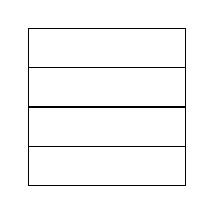
\begin{tikzpicture}
  \draw (0, 0) rectangle (2, 0.5);
  \draw (0, 0.5) rectangle (2, 1);
  \draw (0, 1) rectangle (2, 1.5);
  \draw (0, 1.5) rectangle (2, 2);
\end{tikzpicture}

\section{Instructions}

This sequence of instructions:

\texttt{LDA \#\$0xFF}

\texttt{PHA}

\texttt{PLP}

\noindent Results in \texttt{P} being set to $(\texttt{EF})_{16}$ and not
$(\texttt{FF})_{16}$? Why? Do the \texttt{N} and \texttt{Z} flags get set
based off the current value of \texttt{A} and not from the stack?

\section{Interrupts}

\section{Instructions}

\subsection{Subtract with Carry}

Be careful with the overflow bit.
